\section{Feliratok fordítása}

Miután már lehetőségünk van arra, hogy a felhasználó szavakra történő kattintásait nyomon kövessük, a következő lépés ezek lefordítása a kívánt nyelvre. Ehhez szükségesünk van egy fordító \textit{API}-ra, azaz egy alkalmazásprogramozási felületre, amely segítségével megvalósíthatóvá válik a szavak anyanyelvre való átültetése. Ehhez a \textit{Microsoft Translate API} interfészre esett a választásom, mivel az összes alternatíva közül ez az egyetlen ingyenes, bizonyos karakterszám eléréséig. Az \textit{API} működésének lényege, hogy a videólejátszó alkalmazás interneten keresztül elküldi a megadott címre a fordítani kívánt szót, majd innen egy \textit{JSON} formátumú válasz érkezik, ami tartalmazza az összes információt, -beleértve a fordításokat is- amelyet a szerver képes volt előállítani az elküldött információk alapján.
A szolgáltatás többféle fordítási módot is támogat:
\begin{itemize}[noitemsep]
\item fordítás, azaz több mondatos szövegek fordítása
\item transzliteráció, azaz nem latin betűkészletet használó nyelvek átbetűzése
\item szófordítás, azaz egyes szavak szótárazása
\end{itemize}
Az alkalmazás szempontjából az utóbbi lesz megfelelő, mivel ez a funkció lehetővé teszi egy szóhoz tartozó több fordítás megjelenítését is, amely a felhasználó szókincsének bővítésére rendkívül hasznos.

\subsection{Szerverrel történő kommunikáció}
A szolgáltatás használatához regisztrálást követően igényelnem kellett egy egyedi kulcsot, amely a fiókom azonosítását szolgálja. A \textit{TranslateService.java} osztály valósítja meg az információáramlást szerver és kliens között. Mivel az \textit{API} egy másik URL-en képes nyelvfelismerésre is, ezért az osztályba két publikus metódus került. Egy, amely a kiválasztott nyelv esetén hívódik, egy másik pedig amikor a nyelvfelismerés aktív (\ref{lst:adott_nyelv}). 

%caption=Függvény, amely kiválasztott nyelv esetén hívódik, 
\begin{lstlisting}[language=java, label={lst:adott_nyelv}]
public TranslateResponse[] PostWithGivenLanguages(
    String from,
    String to,
    String string) throws IOException {
        givenLanguageUrl += from + "&to=";
        givenLanguageUrl += to;

        Gson gson = new GsonBuilder()
            .setPrettyPrinting()
            .create();
        return gson.fromJson(createResoponse(string,
            givenLanguageUrl).
        body().string(), TranslateResponse[].class);
    }
\end{lstlisting}
Ebben az esetben a metódus három paraméterrel rendelkezik:
\begin{itemize}[noitemsep]
\item String from, a forrásnyelv
\item String to, a célnyelv
\item String string, a fordítandó szöveg
\end{itemize}
Működése közben előállít egy URL-t, amely tartalmazza a fent említett forrás- és célnyelvet, valamint a felhasználáshoz szükséges kulcsot, beégetett módon. A \textit{createResponse} metódus felelős a szerverrel történő kommunikációért, beleértve a kérés elküldését, illetve a válasz átadását is. A kapott \textit{JSON} formátumú szöveget \textit{Gson} segítségével deszerializálja, így jön létre egy \textit{TranslateResponse} tömb, amely a szervertől kapott választ hivatott reprezentálni. Ez tartalmazza az elérhető fordításokból alkotott listát, mellyel tovább dolgozhatunk.

%caption=Függvény, amely detektált nyelv esetén hívódik, 
\begin{lstlisting}[language=java, label={lst:felismert_nyelv}]
public DetectedLanguageResponse[] PostWithLanguageDetection(
    String string) throws IOException {
        Gson gson = new GsonBuilder()
            .setPrettyPrinting()
            .create();
        return gson.fromJson(createResoponse
            (string,
            "https://api.cognitive.microsofttranslator.com
            /detect?api-version=3.0")
                .body().string(),
            DetectedLanguageResponse[].class);
    }
\end{lstlisting}
A \ref{lst:felismert_nyelv} ábrán látható a detektált nyelv esetén meghívott függvény. Az előző metódushoz képest annyi különbség fedezhető fel, hogy a paraméterlistában csak a lefordítandó szöveg szerepel, és a POST kérés másik címre fut be. Ezen kívül a feldolgozott \textit{JSON} egy \textit{DetectedTranslateResponse}-okat tartalmazó tömbbe kerül. 

\subsection{Fordítások megjelenítése}
\begin{figure}
  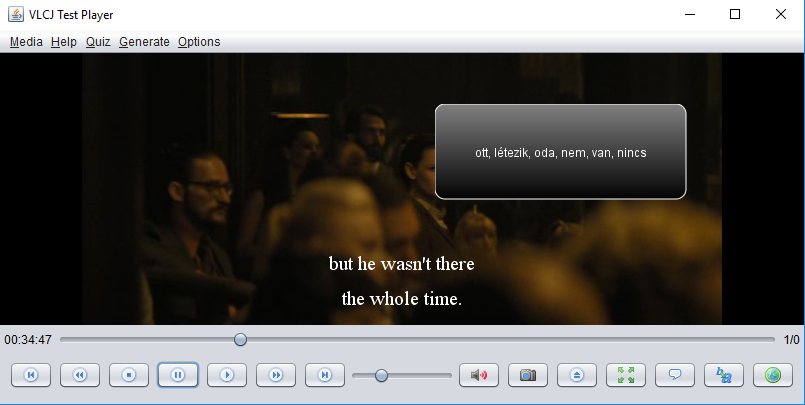
\includegraphics[width=\linewidth]{images/popup.png}
  \caption{A megjelenő felugró ablak}
  \label{fig:popup}
\end{figure}

A fordítások és annak egyéb adatai deszerializáció után kinyerhetők egy-egy objektumtömbből. A következő feladat ezek felhasználóbarát megjelenítése volt. További kritérium, hogy komponens nem szakíthatja meg a videó folytonosságát, illetve nem zavarhatja a nézőt a jelenléte. Mindezek miatt egy felugró ablakot készítettem, amely mondatelemre történő kattintás esetén megjelenik, majd néhány másodperc elteltével eltűnik a képernyőről. Az ablak tartalmazza az aktuális szó összes elérhető fordítását, ha pedig ilyen nem található a \textit{No translations available} felirat jelenik meg. Ennek a megjelenítéséért a \textit{PopupMessageBuilder.java} osztály felelős. Maga az ablak egy \textit{JPanel}-ből származik, melyet a \textit{paintComponent} metódus segítségével rajzol az alkalmazás a képernyőre. A builder osztályt olyan módon készítettem el, hogy segítségével könnyedén, és kényelmesen lehessen felugró ablakokat megjeleníteni a felhasználói a felületen. A \ref{lst:popup}-os ábrán látható módon, pozíció, időtartam, üzenet megadásával jeleníthető meg a komponens. Jelen esetben a kattintás helye felett, három másodperces időtartammal jelenik meg az üzenet, amely a fordítást tartalmazza.

\begin{lstlisting}[caption=A \textit{PopupMessageBuilder} használata, label={lst:popup}, language=java]
new PopupMessageBuilder()
    .at(new Point((int) e.getPoint().getX(), e.getY()
    -(int)(Toolkit.getDefaultToolkit().getScreenSize().height*0.1)))
    .withDelay(3000)
    .withMessage(word.getMeaning())
    .show();

new PopupMessageBuilder()
    .at(new Point((int) e.getPoint().getX(), e.getY()
    -(int) (Toolkit.getDefaultToolkit().getScreenSize().height*0.1)))
    .withDelay(3000)
    .withMessage("No translations available")
    .show();
\end{lstlisting}

A felugró ablak megjelenését filmnézés közben a \ref{fig:popup}-os számú ábrán láthatjuk.